
%%%%%%%%%%%%%%%%%%
% Classification %
%%%%%%%%%%%%%%%%%%

\section{Classification}
\label{sec:class}



% Object classification network %
%%%%%%%%%%%%%%%%%%%%%%%%%%%%%%%%%

\subsection{Object classification networks}
\label{sec:class1}

In this section\footnote{This section's supporting code can be found in \texttt{scripts/itnodl\_class.py} and \texttt{scripts/itnodl\_class\_inc.py}.}, three different classification networks were built and trained, based on the deep convolutional autoencoder model learnt in section \textcolor{blue}{\ref{sec:auto2}}. Specifically, I retained the encoding part of the DCA (from input to encoded layer), and appended layers to allow for classification training. Three approaches were taken with regard to the model parameters:

\begin{enumerate}

	\item{Encoder layers are \textbf{\textsl{frozen}}.}
	\item{Encoder layers are \textbf{\textsl{trainable}}, and \textbf{\textsl{encoder weights are kept from DCA}}.}
	\item{Encoder layers are \textbf{\textsl{trainable}}, and all parameters \textbf{\textsl{train from scratch}}.}

\end{enumerate}

The goal in comparing these approaches is 1) to explore what the value of the previously learnt encoded representation is as a basis for classification, and 2) relatedly, to see whether the pretrained encoder weights serve as a better or worse starting point for classification training. Observation of the class labels shows that the source data represents a \textbf{multi-label} problem---that is, multiple classes can be present in a single image. As such, predictions are considered as a combination of binary labels, rather than a single categorical label. 

\vspace{5mm}

In addition to these three models, two extra models were built. One was \textbf{\textsl{based on the convolutional base layers of the Inception architecture, and pretrained on the ImageNet dataset}}. These base layers were frozen---a similar approach as described with the first model discussed above---and additional fully connected layers were added to facilitate classification. In other words, this model benefits from a more complex architecture, and is fully pretrained on a larger dataset. (The odds are stacked heavily in its favor.)

A second extra model was a simple \textbf{\textsl{combination between the deep convolutional autoencoder and a classification network}}. More specifically, this model reused the DCA architecture, but appended classification-purposed layers to the encoded layer. The model was then jointly trained on the two different task: image reconstruction and image classification.

\begin{figure}[!htbp]
	\begin{center}
		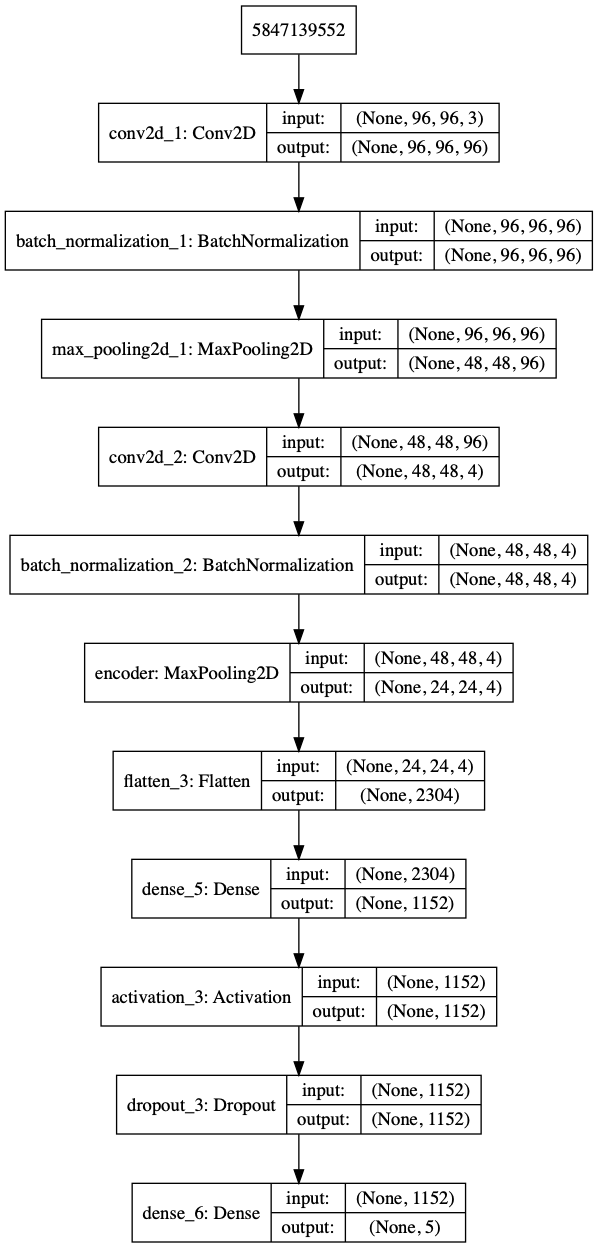
\includegraphics[height=20cm, keepaspectratio]{images/class_architecture}
		\caption{Architecture for the home-cooked classification network. Input dimensions are $96 \times 96\times3$, and the output vector is $5\times1$.}
		\label{fig:class}
	\end{center}
\end{figure}




% Architectures

\paragraph{Architecture} 
The common architecture of the three approaches, apart from the trainability and weight initialization of the parameters, is shown in figure \ref{fig:class}. Several layers were added at the end of the encoder part to allow for classification training. Specifically, the encoded representation was flattened, and passed through two more fully connected layers (Dense layers in Keras). The first of these layers used ReLU, whereas the final layer---containing the classification results---has a sigmoid activation function. Between both layers, dropout was applied. In other words, some of the input to the final layer is dropped out randomly, in an attempt to make the network more robust. The output layer consisted of 5 nodes, to accommodate the K-hot encoded label vector.

\paragraph{Data augmentation} The get the most out of the images at hand, which are in relative low number for the purpose of classification, data augmentation was applied during training. Data augmentation is a technique that simulates additional variability in a dataset by applying minor manipulations, such as rotations or cropping. In this case, the following parameters were applied:

\begin{enumerate}

	\item A 15 degree range was set for random rotations.
	\item A 0.1 range was set for shifts in width.
	\item A 0.1 range was set for shifts in height.
	\item Horizontal flipping was allowed.
	
\end{enumerate}




% Network parameters

\paragraph{Network parameters}
Similar to section \textcolor{blue}{\ref{sec:auto}}, all networks were trained using the \textit{Adam} optimizer algorithm. Several loss functions were experimented with. Results varied, but the comparison between the four presented networks remained fairly consistent. In the remainder of this section, I will discuss results for networks trained using the \textit{binary crossentropy} loss function, as this is the go-to loss function for multi-label classification\footnote{If the problem were multi-class, but not multi-label, the preferred loss function would have been \textit{categorical crossentropy}, combined with a \textit{softmax} activation function in the final layer.}. All model training was set for \textit{300 epochs}. Similar to the approach in section \textcolor{blue}{\ref{sec:auto}}, training \textit{stopped early} if no improvement was detected in the validation loss for a number epochs. In this case, that number was set to 50. 

\begin{figure}[!htbp]
	\begin{center}
		\includegraphics[width=\linewidth, keepaspectratio]{images/class_histories1}
		\caption{Training history for all classifier models. In the top row, the left graph shows the evolution of the accuracy on the training data, whereas the right graph shows the evolution of the validation accuracy. In the bottom row, the graphs represent the evolution of the training and validation loss (\textit{binary crossentropy}). The vertical dotted line indicates when early stopping occurred, due to a lack of improvement in the latter value.}
		\label{fig:class_histories1}
	\end{center}
\end{figure}

\begin{figure}[!htbp]
	\begin{center}
		\includegraphics[width=\linewidth, keepaspectratio]{images/class_metrics1}
		\caption{Evaluation metrics applied to test image classification, for each of the five different modeling approaches.}
		\label{fig:class_metrics1}
	\end{center}
\end{figure}

\paragraph{Evaluation}
%TODO: fix this
All model training stopped (very) early, despite the forgiving stopping criterion (see figure \ref{fig:class_histories1}). This suggests that extended training had little to no impact on the validation loss or accuracy of any of the models. Furthermore, the evolution of the training loss suggests that the difference between the approaches boils down to simple rules: 1) the first approach (frozen encoded layers) rendered the model less flexible, thus inhibiting loss decrease compared to the other models, and 2) it appeared better to let the model learn its own weights from scratch, rather than initializing them to the values that were learnt for the autoencoder problem, and 3) the Inception-based network simply performed better, likely due to the combination of the more advanced architecture and the (costly) pretraining. Interestingly, the strategy learnt during the training phase of the deep convolutional autoencoder (Approach 1: not from scratch, not all layers trainable) did not simply translate to a better (or more rapidly acquired) strategy for the classification problem. On the contrary, it appeared to be more of a hindrance, causing training performance to lag behind a randomized sibling network.

The problem we are dealing with here is of the \textbf{multi-class, multi-label} classification variety. Our architecture deals with this by treating every label independently. In some sense, we are treating the problem as multiple binary classification problems rather than a single categorical classification task. This causes the accuracy calculated by Keras, which is also shown in the figures, to be inflated. Since most images have one, maximum two positive labels, the vast majority of target values is 0. This means that a model that consistently predicts 0 outcomes is likely to be considered fairly 'accurate' by the default metric, even though no strategies are learnt. We thus require better evaluation metrics that account for this inflation problem.

Here, several multi-label classification metrics were used to evaluate the different models. They were calculated based on the previously unseen test images. Figure \ref{fig:class_metrics1} shows the scores and rankings of each of the models. Where there was a choice, the \textit{macro-average} of the metric was used, rather than the \textit{micro-average}. The former approach computes the metric independently for each class, and returns the average. The micro-average combines the contributions per class to compute the average metric.  In a multi-class classification setup, micro-average is preferable if you suspect there might be class imbalance (i.e you may have many more examples of one class than of other classes. This was not the case.

\begin{itemize}
 	\item{\textbf{Exact match ratio} represents the proportion of target vectors that got predicted exactly, meaning each of the prediction node values matched their respected target values. \textit{Higher values are better.}}
	\item{\textbf{$F_1$-score} represents the harmonic average of them model's precision and recall. Calculated globally using the total amount of true positives, false negatives and false positives. \textit{Higher values are better.}}
	\item{\textbf{Hamming loss} is defined as the fraction of labels that are incorrectly predicted. \textit{Lower values are better.}}
	\item{\textbf{Hamming score} is calculated as the number of correct labels divided by the union of predicted and true labels. \textit{Higher values are better.}}
	\item{\textbf{Jaccard similarity score} compares members for two sets ---the predicted labels and true labels---to see which members are shared and which are distinct. \textit{Higher values are better.}}
\end{itemize}

Inspection of the metrics (figure \ref{fig:class_metrics1} suggests that---among these first three models---the third approach was most effective at creating an accurate model, followed closely by the second approach (all layers trainable and starting weights randomized). This is primarily evident in the higher $F_1$-score and the slightly lower Hamming loss.  The first approach (frozen encoder layers) underperformed in comparison, suggesting that the feature representation learned by autoencoders is not directly transferable to the classification problem setting.

\begin{figure}[!htbp]
	\begin{center}
		\includegraphics[width=\linewidth, keepaspectratio]{images/class_histories1_long}
		\caption{Training history for all classifier models. In the top row, the left graph shows the evolution of the accuracy on the training data, whereas the right graph shows the evolution of the validation accuracy. In the bottom row, the graphs represent the evolution of the training and validation loss (\textit{binary crossentropy}). The vertical dotted line indicates when early stopping occurred, due to a lack of improvement in the latter value.}
		\label{fig:class_histories1_long}
	\end{center}
\end{figure}



\paragraph{Expansion on homemade models}
Because little to no improvement was found in validation accuracy and loss (and since this came across as suspicious) the early stopping criterion was removed from the home-made model training. This decision was made to verify the longer term effects of training. However, even with extended training duration (see figure \ref{fig:class_histories1_long}), no evidence was found of a(n eventual) positive impact on validation accuracy and loss. On the contrary, it seemed as though any improvement in training loss came at the cost of an increase in validation loss, suggesting overtraining. The models thus became increasingly better at handling the training data---especially in the third approach, with all trainable layers and randomized starting weights---but no generally applicable strategy was learnt. In an attempt to better these unsatisfactory results, new modeling approaches were undertaken. They are described in the next sections.




% Inception-based classification network %
%%%%%%%%%%%%%%%%%%%%%%%%%%%%%%%%%%%%%%%%%%

\subsection{Inception-based classification}

Inception is an image recognition model designed by researchers at Google. It was specifically developed to solve problems in the field of Computer Vision. The architecture is notable for its leveraging of various ideas, old and new, into a performant new breed of neural network. 

\begin{figure}[!htbp]
	\begin{center}
		\includegraphics[width=10cm, keepaspectratio]{images/class_inc_architecture}
		\caption{Architecture for the Inception-based classification network. Input dimensions are $96\times 96\times3$, and the output vector is $5\times1$. }
		\label{fig:class_inc}
	\end{center}
\end{figure}

\paragraph{Architectures} 
The architecture of the Inception classifier is visualized in figure \ref{fig:class_inc}. The convolutional base was taken from the InceptionResNetV2 architecture (as it is implemented in Keras), with input dimensions $96\times 96\times3$. The underlying architecture for these base layers is described \textcolor{blue}{\href{https://github.com/WouterDurnez/003_FinalProject} {here\footnote{https://arxiv.org/pdf/1512.00567v3.pdf}}}. The model base was pre-trained on the ImageNet database. Similar to the architectures described above, two fully connected layers were added to the model to allow for classification training.


\paragraph{Network parameters} The model was trained using the same parameter settings as described in previous section: it trained for \textit{300 epochs} with \textit{early stopping} set at 50, using the \textit{Adam} optimizer function and \textit{binary crossentropy} as loss function. Data augmentation was used during training, similar to what was described in \ref{sec:class1}.

\begin{figure}[!htbp]
	\begin{center}
		\includegraphics[width=\linewidth, keepaspectratio]{images/class_histories2}
		\caption{Training history for the Inception-based classification model (\textcolor{red}{red}). The previous models are shown as a reference. The vertical dotted line indicates when early stopping occurred.}
		\label{fig:class_histories2}
	\end{center}
\end{figure}

\paragraph{Evaluation}
Figure \ref{fig:class_histories2} depicts the training progression of the Inception-based model. It appears as though the model learnt all it could fairly quickly, after which loss and accuracy stabilized. In that sense, it is similar our the first model (frozen encoder layers): the basis for feature extraction was set (and could not be changed), and the classification layers optimized in short term. In addition, it is clear that validation accuracy is distinctly higher for the Inception-based network. This is likely the result of the pre-training advantage the network was endowed with, illustrating the value of large amounts of training data in deep learning. Evaluation of the final model is shown in \ref{fig:class_metrics2}. Again, it is clear that the Inception-based model is our most performant model thus far. This can be seen in the lesser Hamming loss, the greater $F_1$-score, and the model's ability to generate a fraction more exact matches.

\begin{figure}[!htbp]
	\begin{center}
		\includegraphics[width=\linewidth, keepaspectratio]{images/class_metrics2}
		\caption{Evaluation metrics for Inception-based classification network. Previous approaches are shown as a reference.}
		\label{fig:class_metrics2}
	\end{center}
\end{figure}




% Joint-trained network %
%%%%%%%%%%%%%%%%%%%%%%%%%

\subsection{Jointly-trained classification network}

To explore the advantage of joint training---i.e. building a network for two separate purposes and training it on both at the same time--a final network was built. Here, the network attempts to both reconstruct and classify an image, based on the deep convolutional autoencoder principle (section \textcolor{blue}{\ref{sec:auto2}}). The network's loss is defined as the sum of the losses calculated on both network outputs. Training attempts to minimize this joint loss, \textit{agnostic to the components it is made out of}.


\begin{figure}[!htbp]
	\begin{center}
		\includegraphics[height=18cm, keepaspectratio]{images/class_joint_architecture}
		\caption{Architecture for the jointly-trained network. Input dimensions are $96\times 96\times3$, and the output consists of both a $96\times 96\times3$ image reconstruction matrix, and a $5\times1$ classification vector. }
		\label{fig:class_joint}
	\end{center}
\end{figure}

\paragraph{Architectures} 
This section's architecture is shown in figure \ref{fig:class_joint}. The model was fed $96\times 96\times3$ images, and returned an attempted image reconstruction matrix of equal dimensions, as well as a classification vector (dimensions $5 \times $1).


\paragraph{Network parameters} The model was trained using the same parameter settings as described in previous section: it trained for \textit{300 epochs} with \textit{early stopping} set at 50, using the \textit{Adam} optimizer function and \textit{binary crossentropy} as loss function.

\begin{figure}[!htbp]
	\begin{center}
		\includegraphics[width=\linewidth, keepaspectratio]{images/class_histories3}
		\caption{Training history for the Inception-based classification model (\textcolor{red}{red}). The previous models are shown as a reference. The vertical dotted line indicates when early stopping occurred.}
		\label{fig:class_histories3}
	\end{center}
\end{figure}

\paragraph{Evaluation}
Inspection of both the validation loss and accuracy (\ref{fig:class_histories3}), as well as the metrics yielded by the final model (\ref{fig:class_metrics3}), suggests that the classifier that resulted from our joint training approach is of little value. While this approach appeared to boost training greatly, the strategies learnt did not translate to the validation data.  On the contrary: while training loss decreased seemingly exponentially, validation loss exploded. Interestingly (though not depicted in the figure), the autoencoder part of the network benefitted from a similar boost. In this case, however, the decrease in loss could also be seen in the validation data. This suggests that it is useful to implement such joint training approach for the purpose of image reconstruction, but not for classification. 


\begin{figure}[!htbp]
	\begin{center}
		\includegraphics[width=\linewidth, keepaspectratio]{images/class_metrics3}
		\caption{Evaluation metrics for Inception-based classification network. Previous approaches are shown as a reference.}
		\label{fig:class_metrics3}
	\end{center}
\end{figure}


\begin{figure}[!htbp]
	\begin{center}
		\includegraphics[width=\linewidth, keepaspectratio]{images/class_prediction_comparison}
		\caption{Classification scores for each of the class labels, generated by each model for a set of test images. Values over 0.5 (dotted line) would be considered a 'detection'.}
		\label{fig:class_prediction}
	\end{center}
\end{figure}



% Reflection %
%%%%%%%%%%%%%%


\subsection{Reflection}
For the most part, the models presented in this section clearly have limited use beyond the training data. The Inception-based model appears to have most predictive value. There are a several possible explanations for this failure.

\begin{itemize}

	\item{With respect to the autoencoder-based models, it is entirely possible that the model architecture was simply not adequate to capture the relevant information needed to classify the images correctly. If it in fact did succeed in capturing relevant information, this 'relevancy' may have been uniquely suited for the reconstruction problem, which is different from the classification problem.}
	
	\item{Given the limited number of training images per class (see table \ref{tab:classcounts}), it is possible that the model did not see enough examples to be able to extract recurring semantic features. The problem could be simplified into a binary classification task, to reduce its complexity. Alternatively, additional images could be sought and added to the training data corpus (we could steal some from the validation set).}
	
	\item{Perhaps \textit{binary crossentropy} is not the most efficient loss function for this sort of problem. In the case of multi-label classification, the loss function appears to suffer from inflation, as it is based on the individual output node values. Alternatively, it may be more effective (but computationally not more efficient) to instantiate a separate model for each class. The multi-label classification problem then becomes set of binary classification problems. This way, the weights of each model can adjust themselves separately, specifically learning strategies to detect a single class.}

\end{itemize}
